\chapter{VNT Evaluation Method}
\label{vnt_evaluation_method}
Once we have the output of the tool in JSON format, it is easy to convert it to other formats to do an analysis of the results or obtain some statistics. 
\section{Calculating the Number of Vulnerabilities}
The python script \texttt{vnt\_format.py} receives the JSON description of VNT results as an input and generates an output in text format describing each vulnerability in one line. This text output can be used by various command line tools, such as grep, cut, etc., to obtain statistics. 
Each line is in the following format:
\begin{framed}

\texttt{c|n;%published\_date;last\_modified\_date;reported\_date;cve\_id;nvd\_description\_url;
cvss\_score;%cpe\_names;
wad\_names
%;
%changed\_field\%old\_value\%new\_value
}

\end{framed}
The first component describes if the vulnerability is new (n) or has changed (c). If there are multiple entries in one component, i.e multiple WAD names, entries are separated by comma.
\\
For Example:
\begin{framed}
\texttt{c;6.8;Red Hat,Fedora,JBoss Web,OpenSSL}
\end{framed}
describes a vulnerability that has changed, has a CVSS score of 6.8 and matches with WAD names `Red Hat', `Fedora', `JBoss Web' and `OpenSSL'.
The following command will output the number of new vulnerabilities and changes in vulnerabilities using the TEXT description of all the results. 
\begin{framed}
\begin{verbatim}
$ cat *.txt| cut `-d;' -f1| sort| uniq -c
\end{verbatim}
\end{framed}
In order to get the critical vulnerabilities one can use the following command:
\begin{framed}
\begin{verbatim}
$ cat *.txt| grep `;\([6-9]\|10\)\.'| cut `-d;' -f1| sort|\
  uniq -c
\end{verbatim}
\end{framed}
It is also important to know the number of vulnerabilities that affect CERN. For this purpose WAD can be used to generate a file with all WAD names used at CERN (one name per line) and then using the following command can give us the same statistics as before, but only considering the vulnerabilities that affect CERN.
\begin{framed}
\begin{verbatim}
$ cat *.txt| grep -f wad_names_at_cern.txt| cut `-d;' -f1|\
  sort| uniq -c
\end{verbatim}
\end{framed}
\begin{framed}
\begin{verbatim}
$ cat *.txt| grep -f wad_names_at_cern.txt|\
  grep `;\([6-9]\|10\)\.'| cut `-d;' -f1| sort|\
  uniq -c
\end{verbatim}
\end{framed}
%
%
\chapter{Implementation Details}
\label{implementation-details}
\section{Vulnerability Notification Tool}

Figure \ref{figure:vnt-internal-arch} illustrates the internal architecture of VNT. 
As you can see there are 2 classes and four scripts in the tool. Class Vulnerability represents vulnerabilities with all their NVD reported fields. 
Class Product takes care of everything that is related to CPE names. The main method in this class is the \texttt{guess\_wad\_names()} method which implements the mapping algorithm. 
Different mapping algorithms were tested and all of them are implemented in this class, however the best one was chosen to be called when mapping was necessary. \texttt{vnt-init.sh} is a shell script that can be used to initialize the tool when it is being deployed on a new machine. This script downloads yearly feeds from NVD and stores all the vulnerability data, so that in future executions, the tool can discover new or updated vulnerabilities. \texttt{send-notification.sh} is the main script of the tool, in the sense that it uses both main components of VNT (VNT\_CORE and VNT\_EMAIL) to download the feeds and report vulnerabilities.
\paragraph{}
VNT needs to have WAD names (apps.txt) to match CPE names to WAD names and WAD findings at CERN (wad\_finidings\_cern.txt) to filter out the irrelevant vulnerabilities. These two text files were generated using WAD. 
\begin{figure}[H]
  \centering
    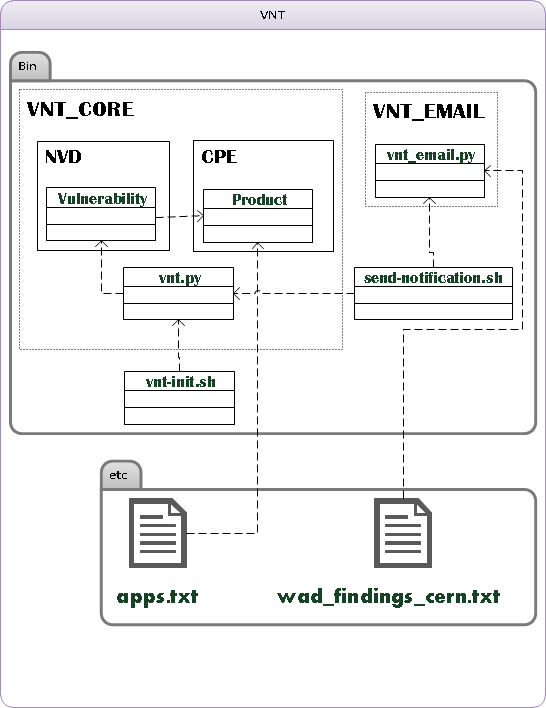
\includegraphics[width=1.0\textwidth]{vnt-internal-arch}
  \caption{VNT Internal Architecture}
   \label{figure:vnt-internal-arch}
\end{figure}

\paragraph{}
Python 2.6 was used as the main programming language for this project (except for the shell scripts) and a total of 1,026 lines of code were developed for this tool. 
\section{Scanner}
Figure \ref{figure:scanner-internal-arch} illustrates the internal architecture of the Scanner. The Scanner is using 4 main Python classes to represent targets, plugins, plugins output and scan results. \texttt{scanner.py} is the main script of the tool to execute when scanning targets. The Scanner is dependent on the available plugins. In order to be able to test the Scanner, it was necessary to develop some plugins or modify the existing ones to follow the Scanner conventions. For this purpose, the plugin \texttt{landing\_page.py} for both websites and servers and \texttt{weak\_cipher.py} for web servers were modified. Also, two other plugins (\texttt{detect\_ssl2.py} and \texttt{detect\_ssl3.py}) were developed by other members of the CERN Computer Security Team to detect if a server is using SSL version 2 or 3 and these scripts were used to test the Scanner.
\begin{figure}[h!]
  \centering
    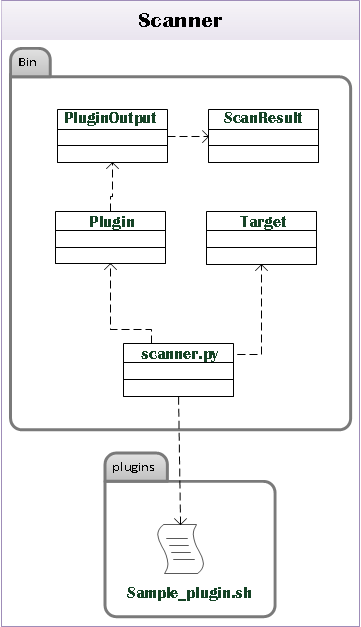
\includegraphics[width=1.0\textwidth]{scanner-internal-arch}
  \caption{Scanner Internal Architecture}
   \label{figure:scanner-internal-arch}
\end{figure}
\paragraph{}
In total, the Scanner contains 977 lines of Python code (without considering the plugins). 